\section{Estrutura}

\subsection{Arquitetura da estrutura}
A estrutura da transportadora de órgãos será feita considerando como principais fatores a  mobilidade e a capacidade de comportar todos os sistemas cumprindo os requisitos de projeto. Além disso, desejou-se aproximar o centro de massa o mais no centro possível da estrutura geral para gerar estabilidade.

Os esquemáticos a seguir mostram de forma simplificada as dimensões, composição e disposição dos elementos estruturais.

\begin{figure}[H]
\centering
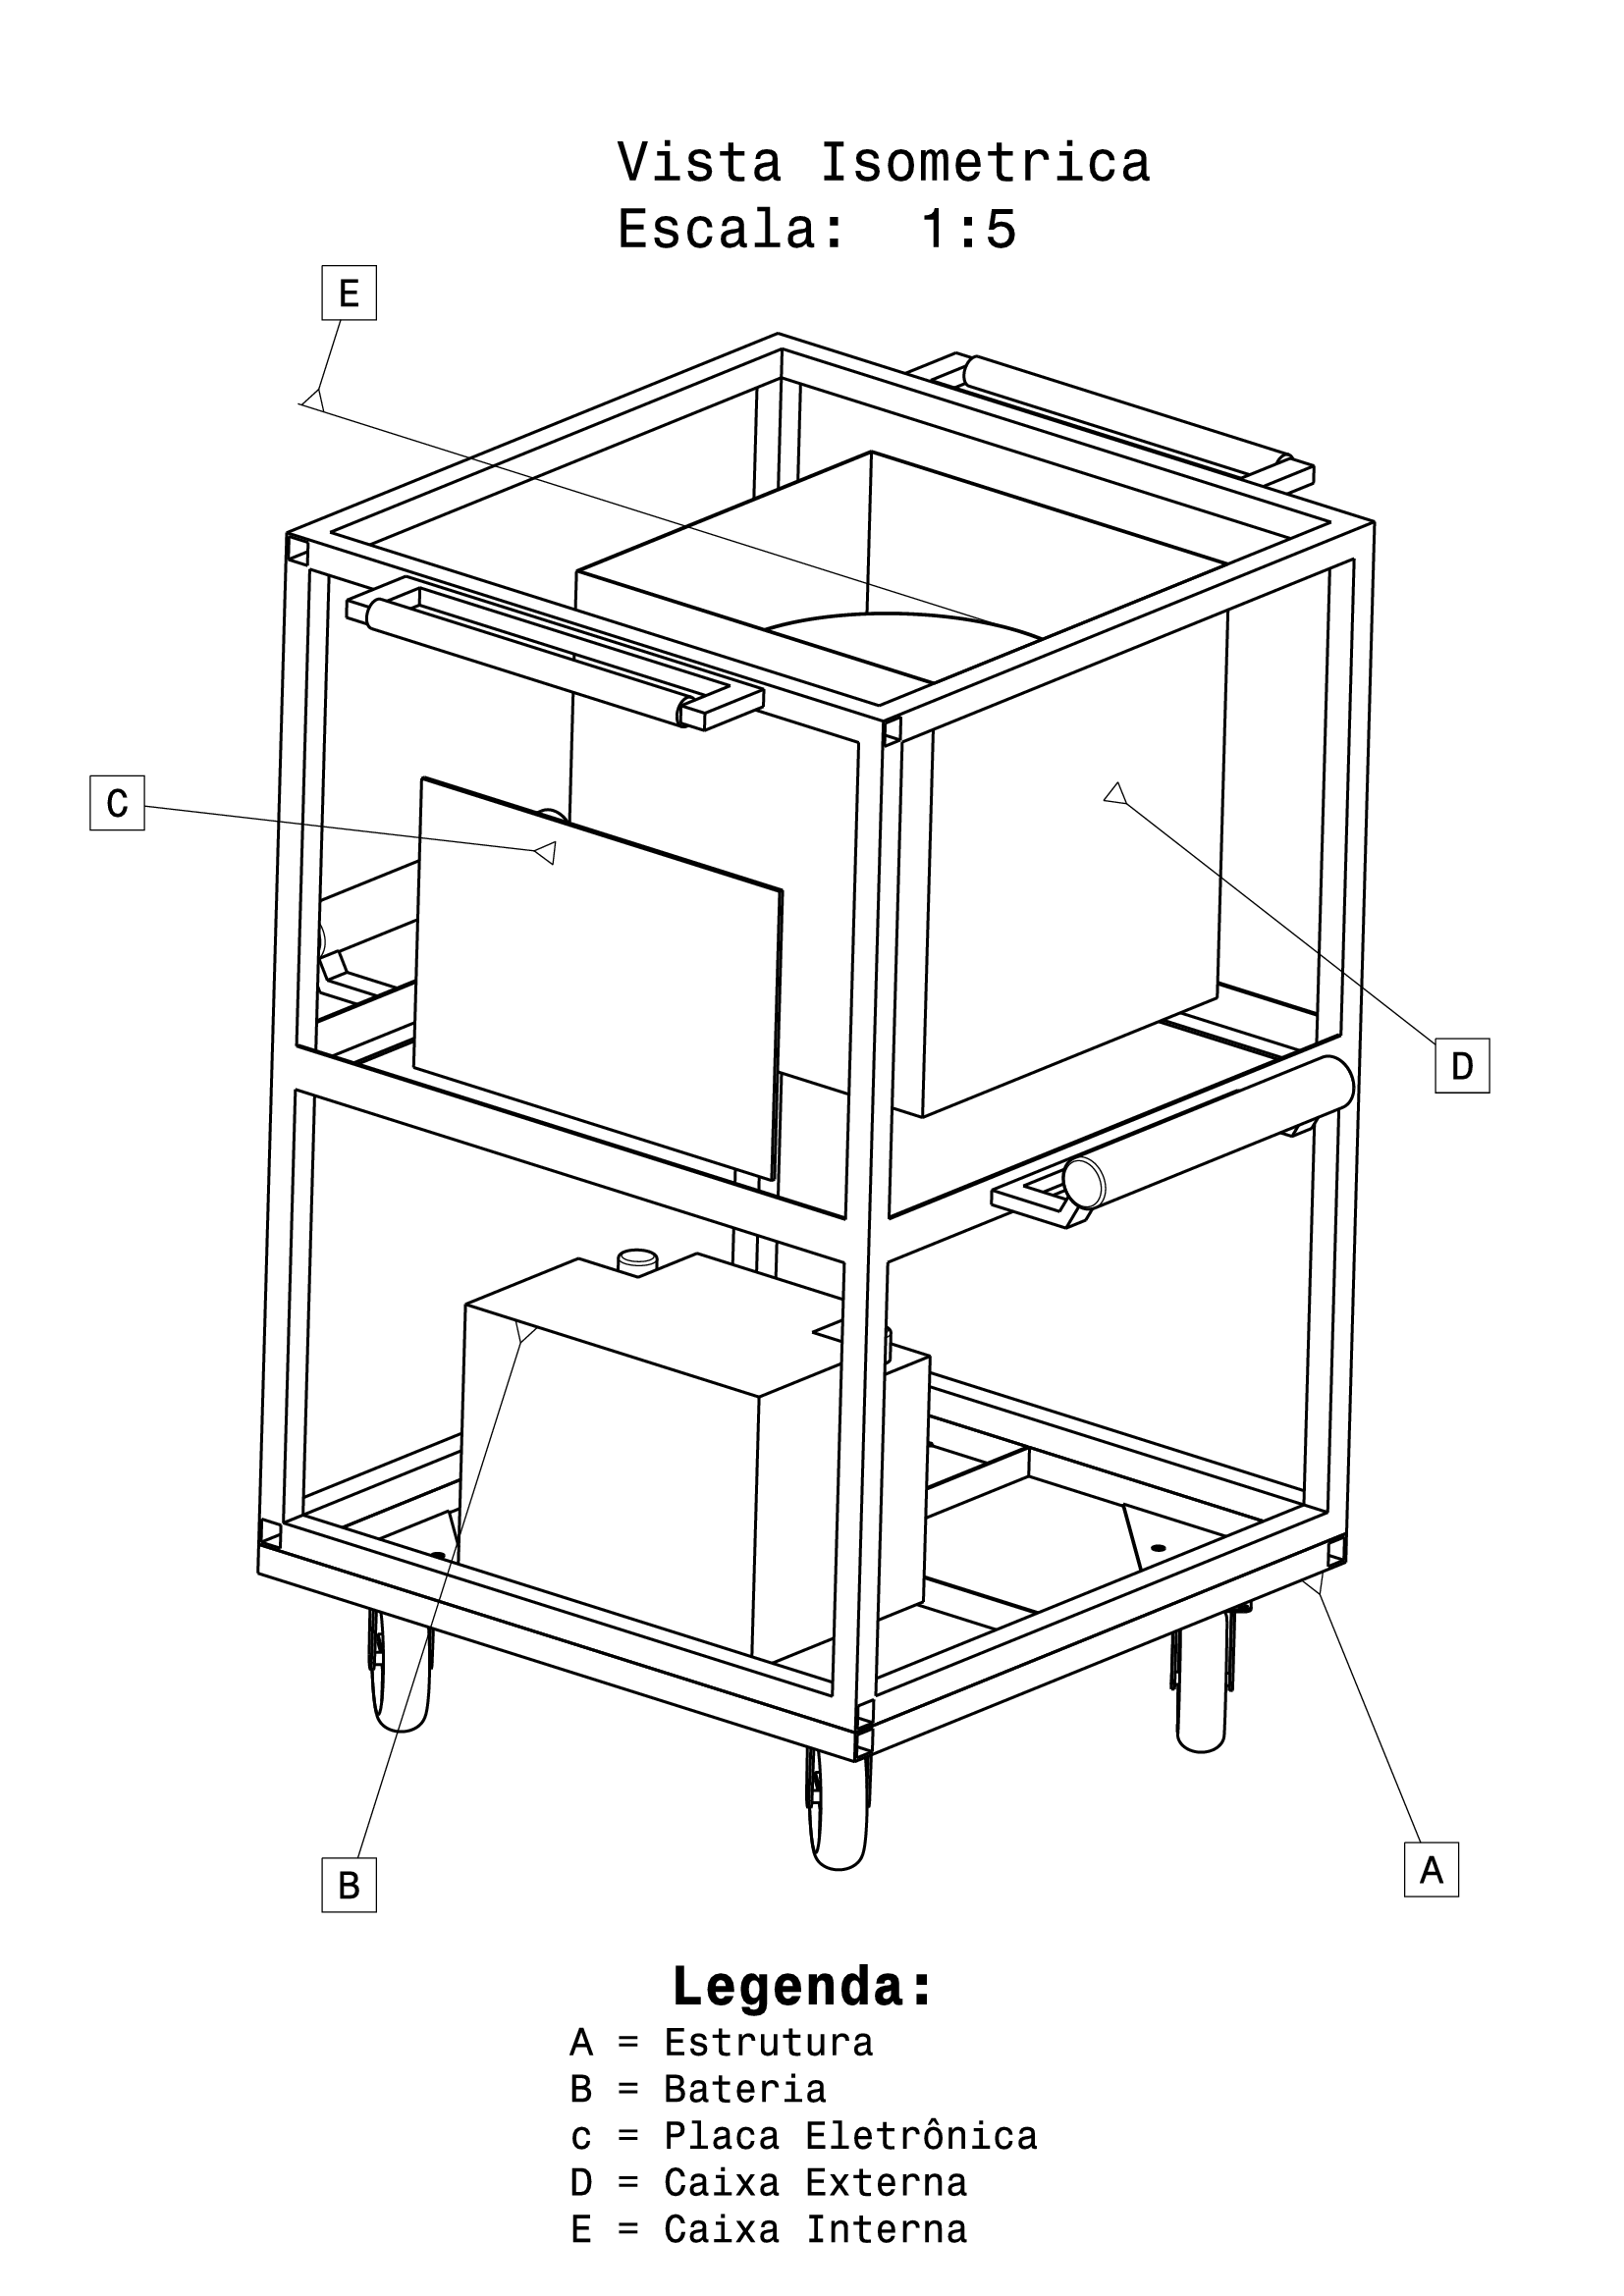
\includegraphics[scale=0.15]{figuras/estrutura.png}
\caption{Estrutura básica da transportadora de órgãos}
\end{figure}

\begin{figure}[H]
\centering
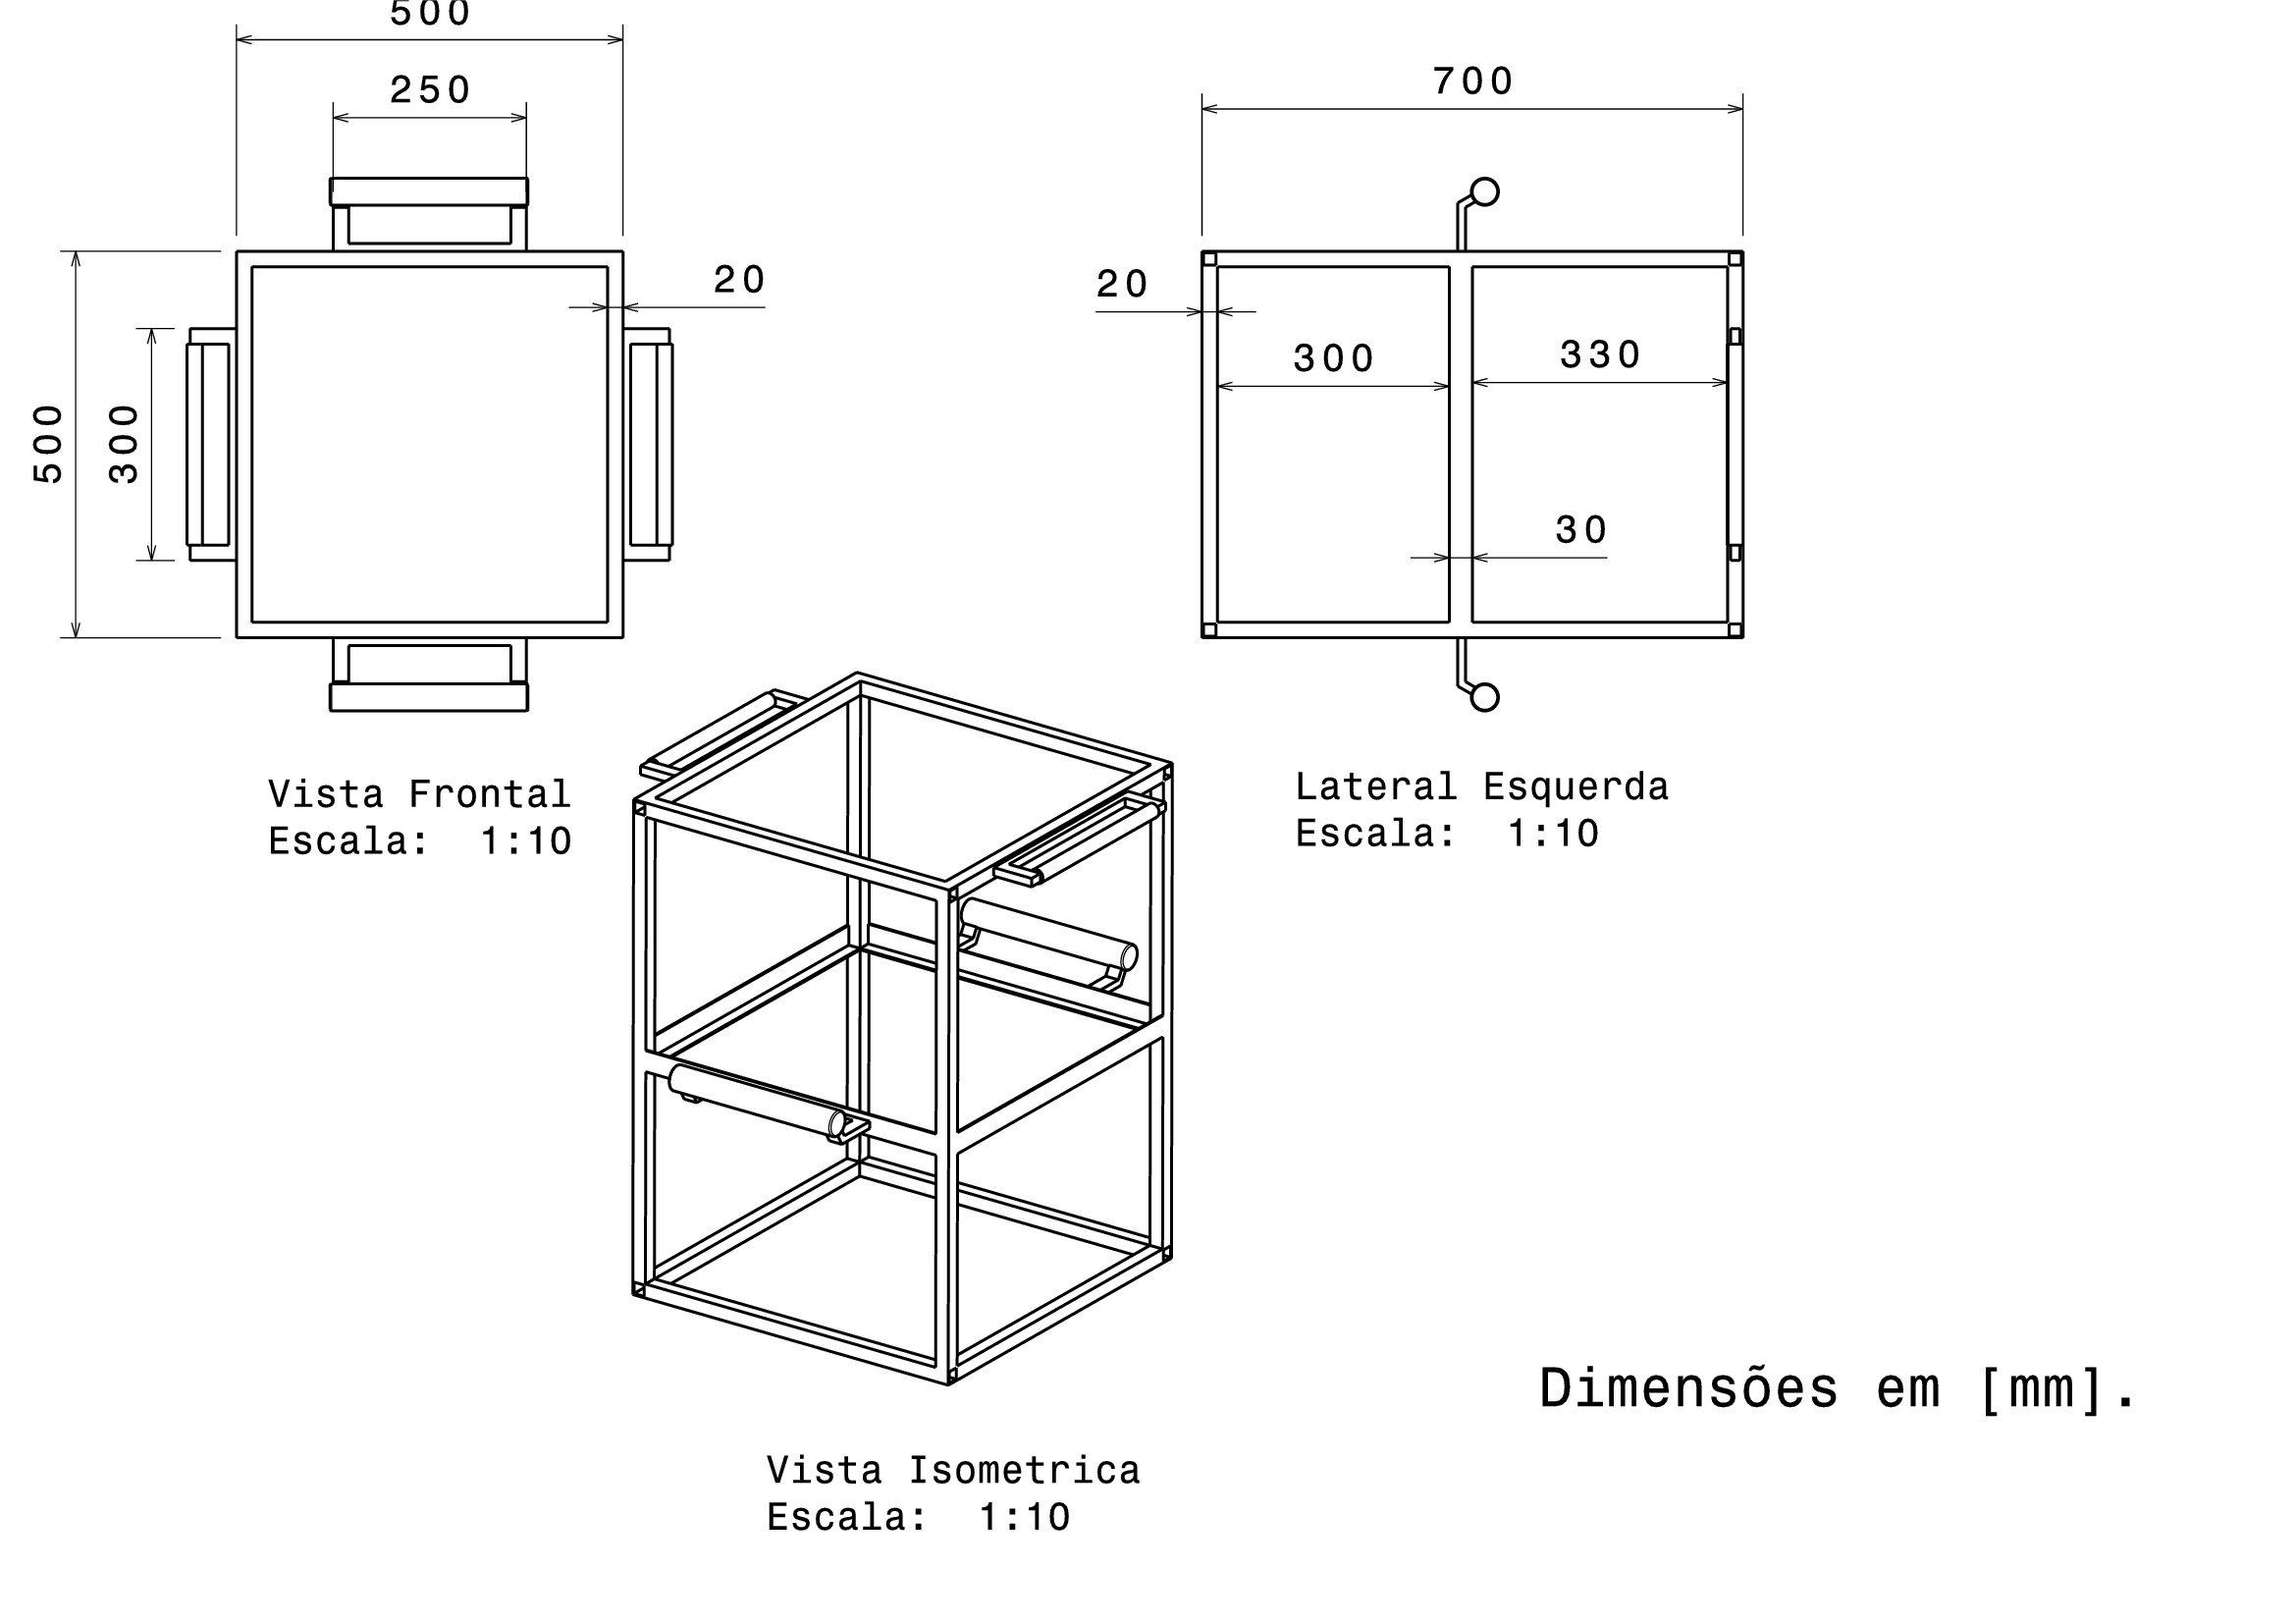
\includegraphics[scale=0.15]{figuras/caixote.png}
\caption{Dimensões da estrutura principal do carrinho}
\end{figure}

\begin{figure}[H]
\centering
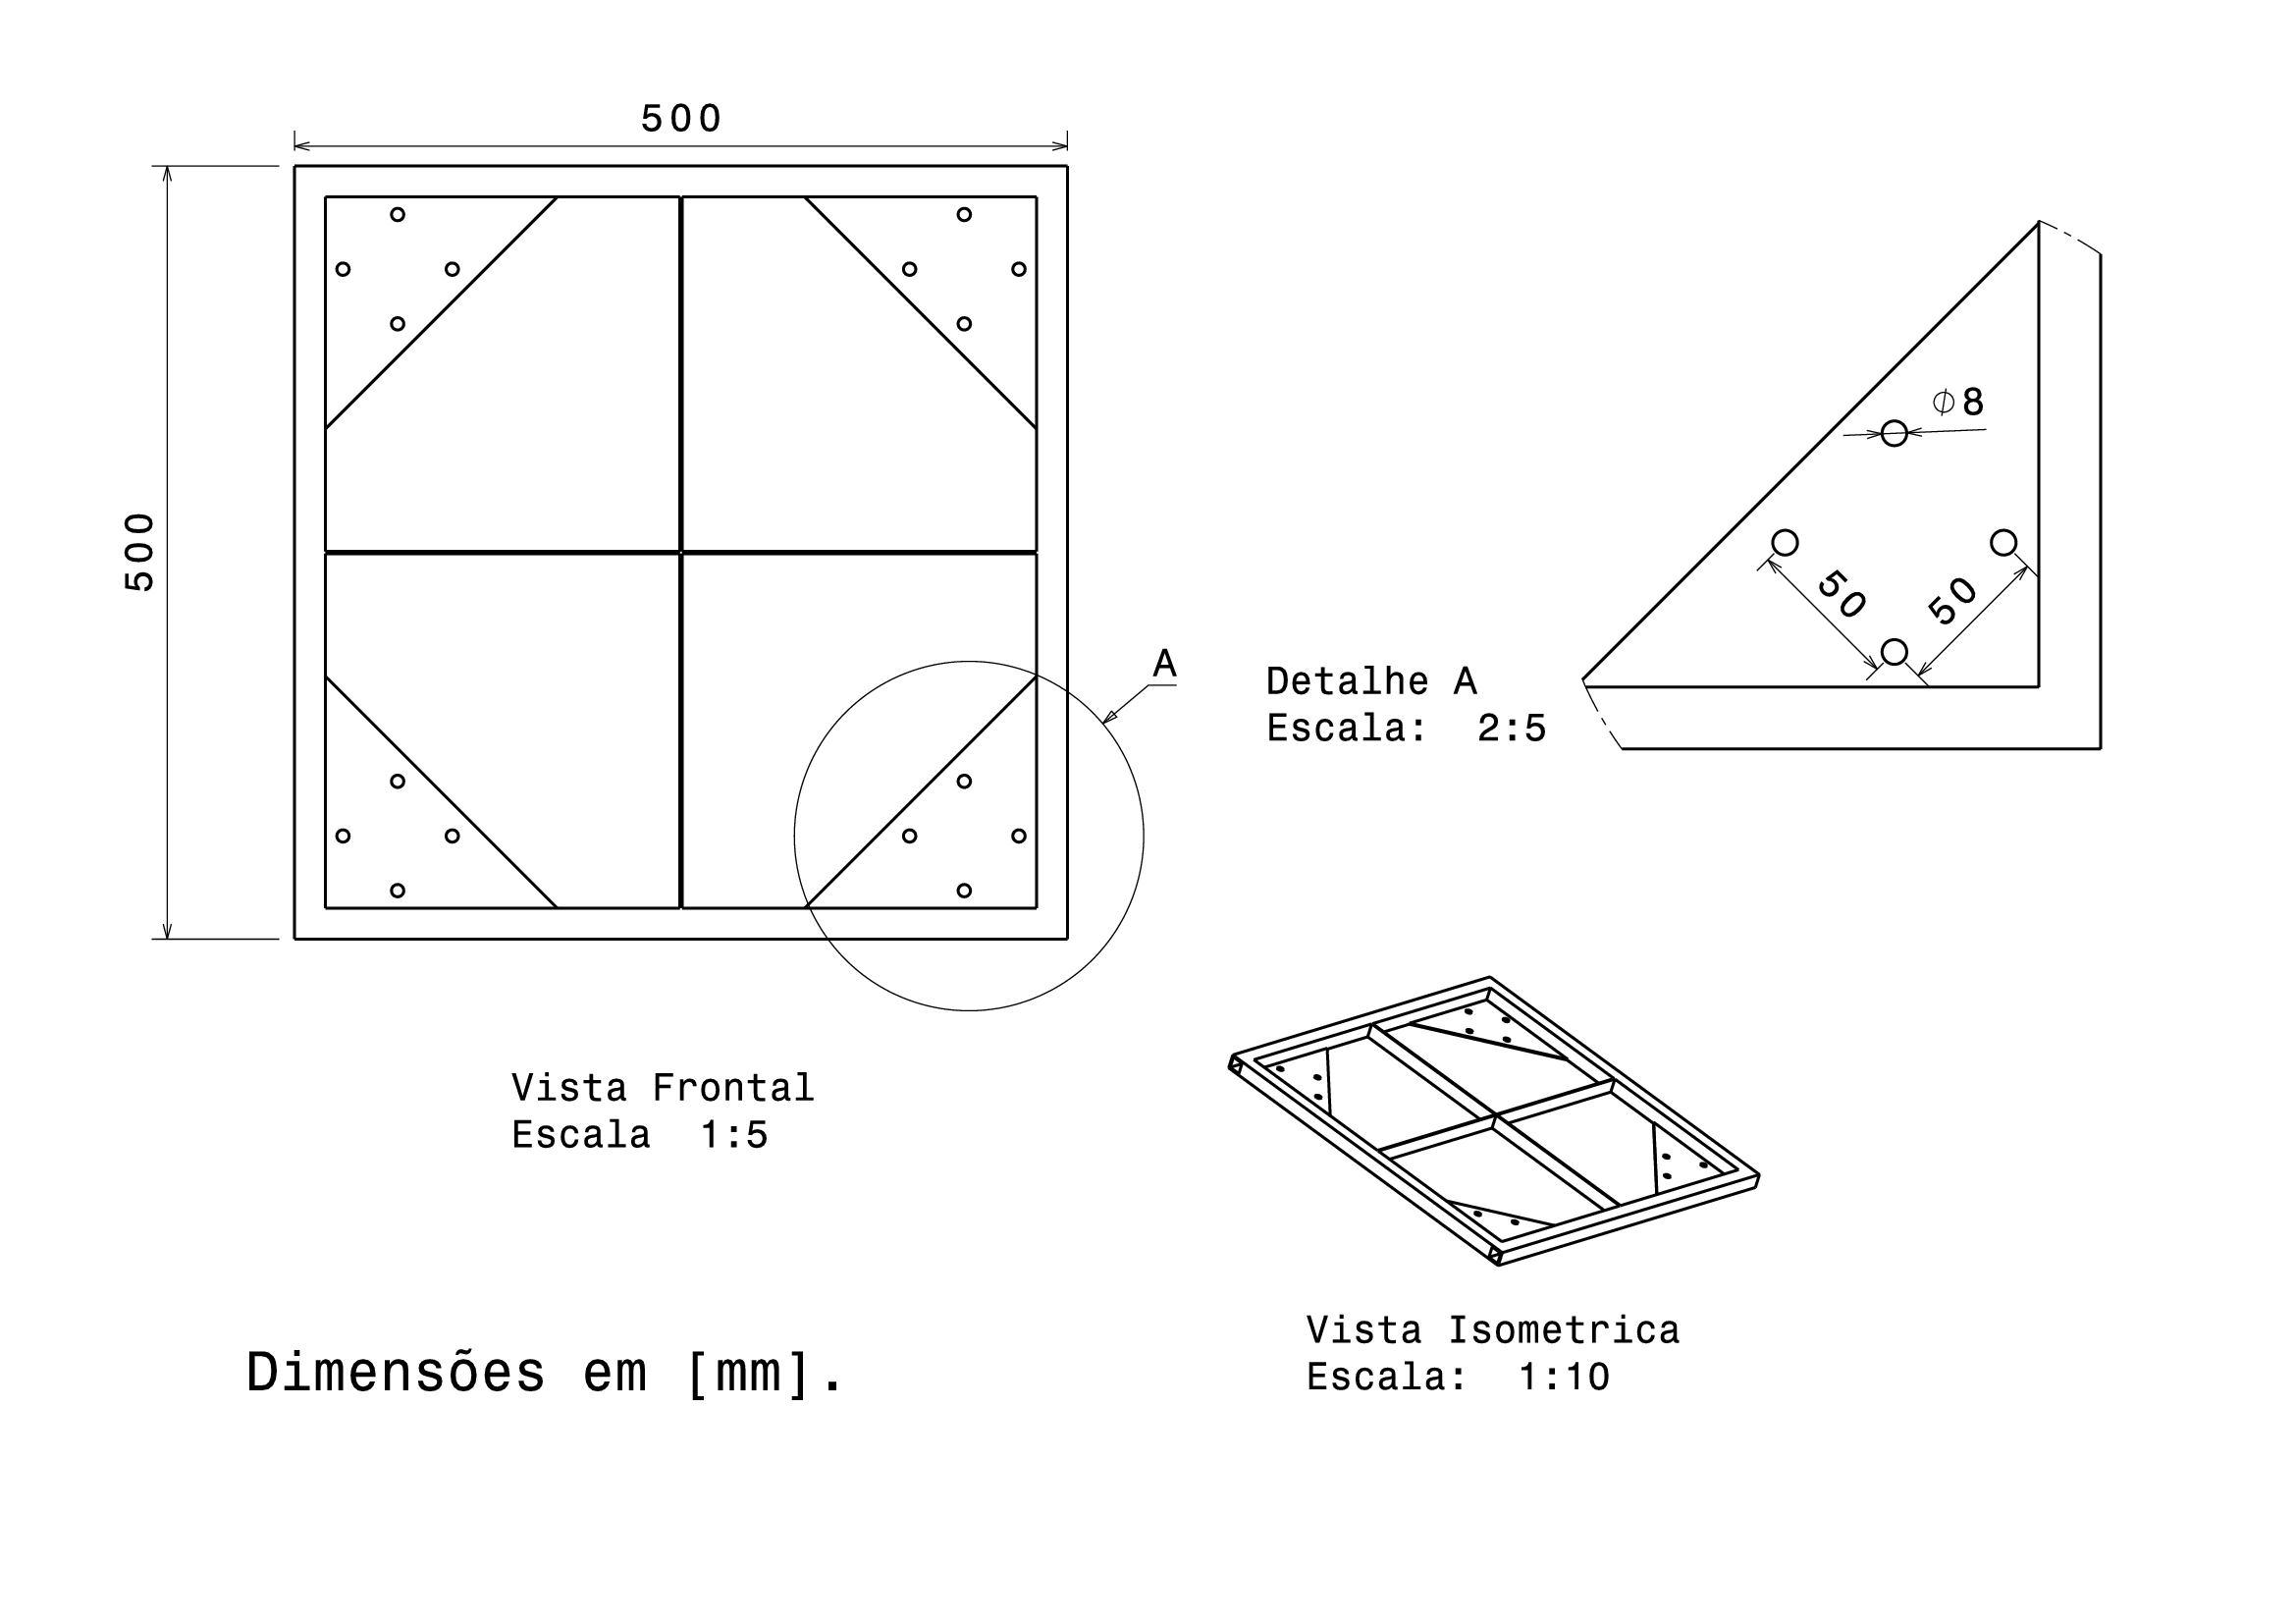
\includegraphics[scale=0.15]{figuras/base.png}
\caption{Dimensões da base de apoio da estrutura}
\end{figure}

\begin{figure}[H]
\centering
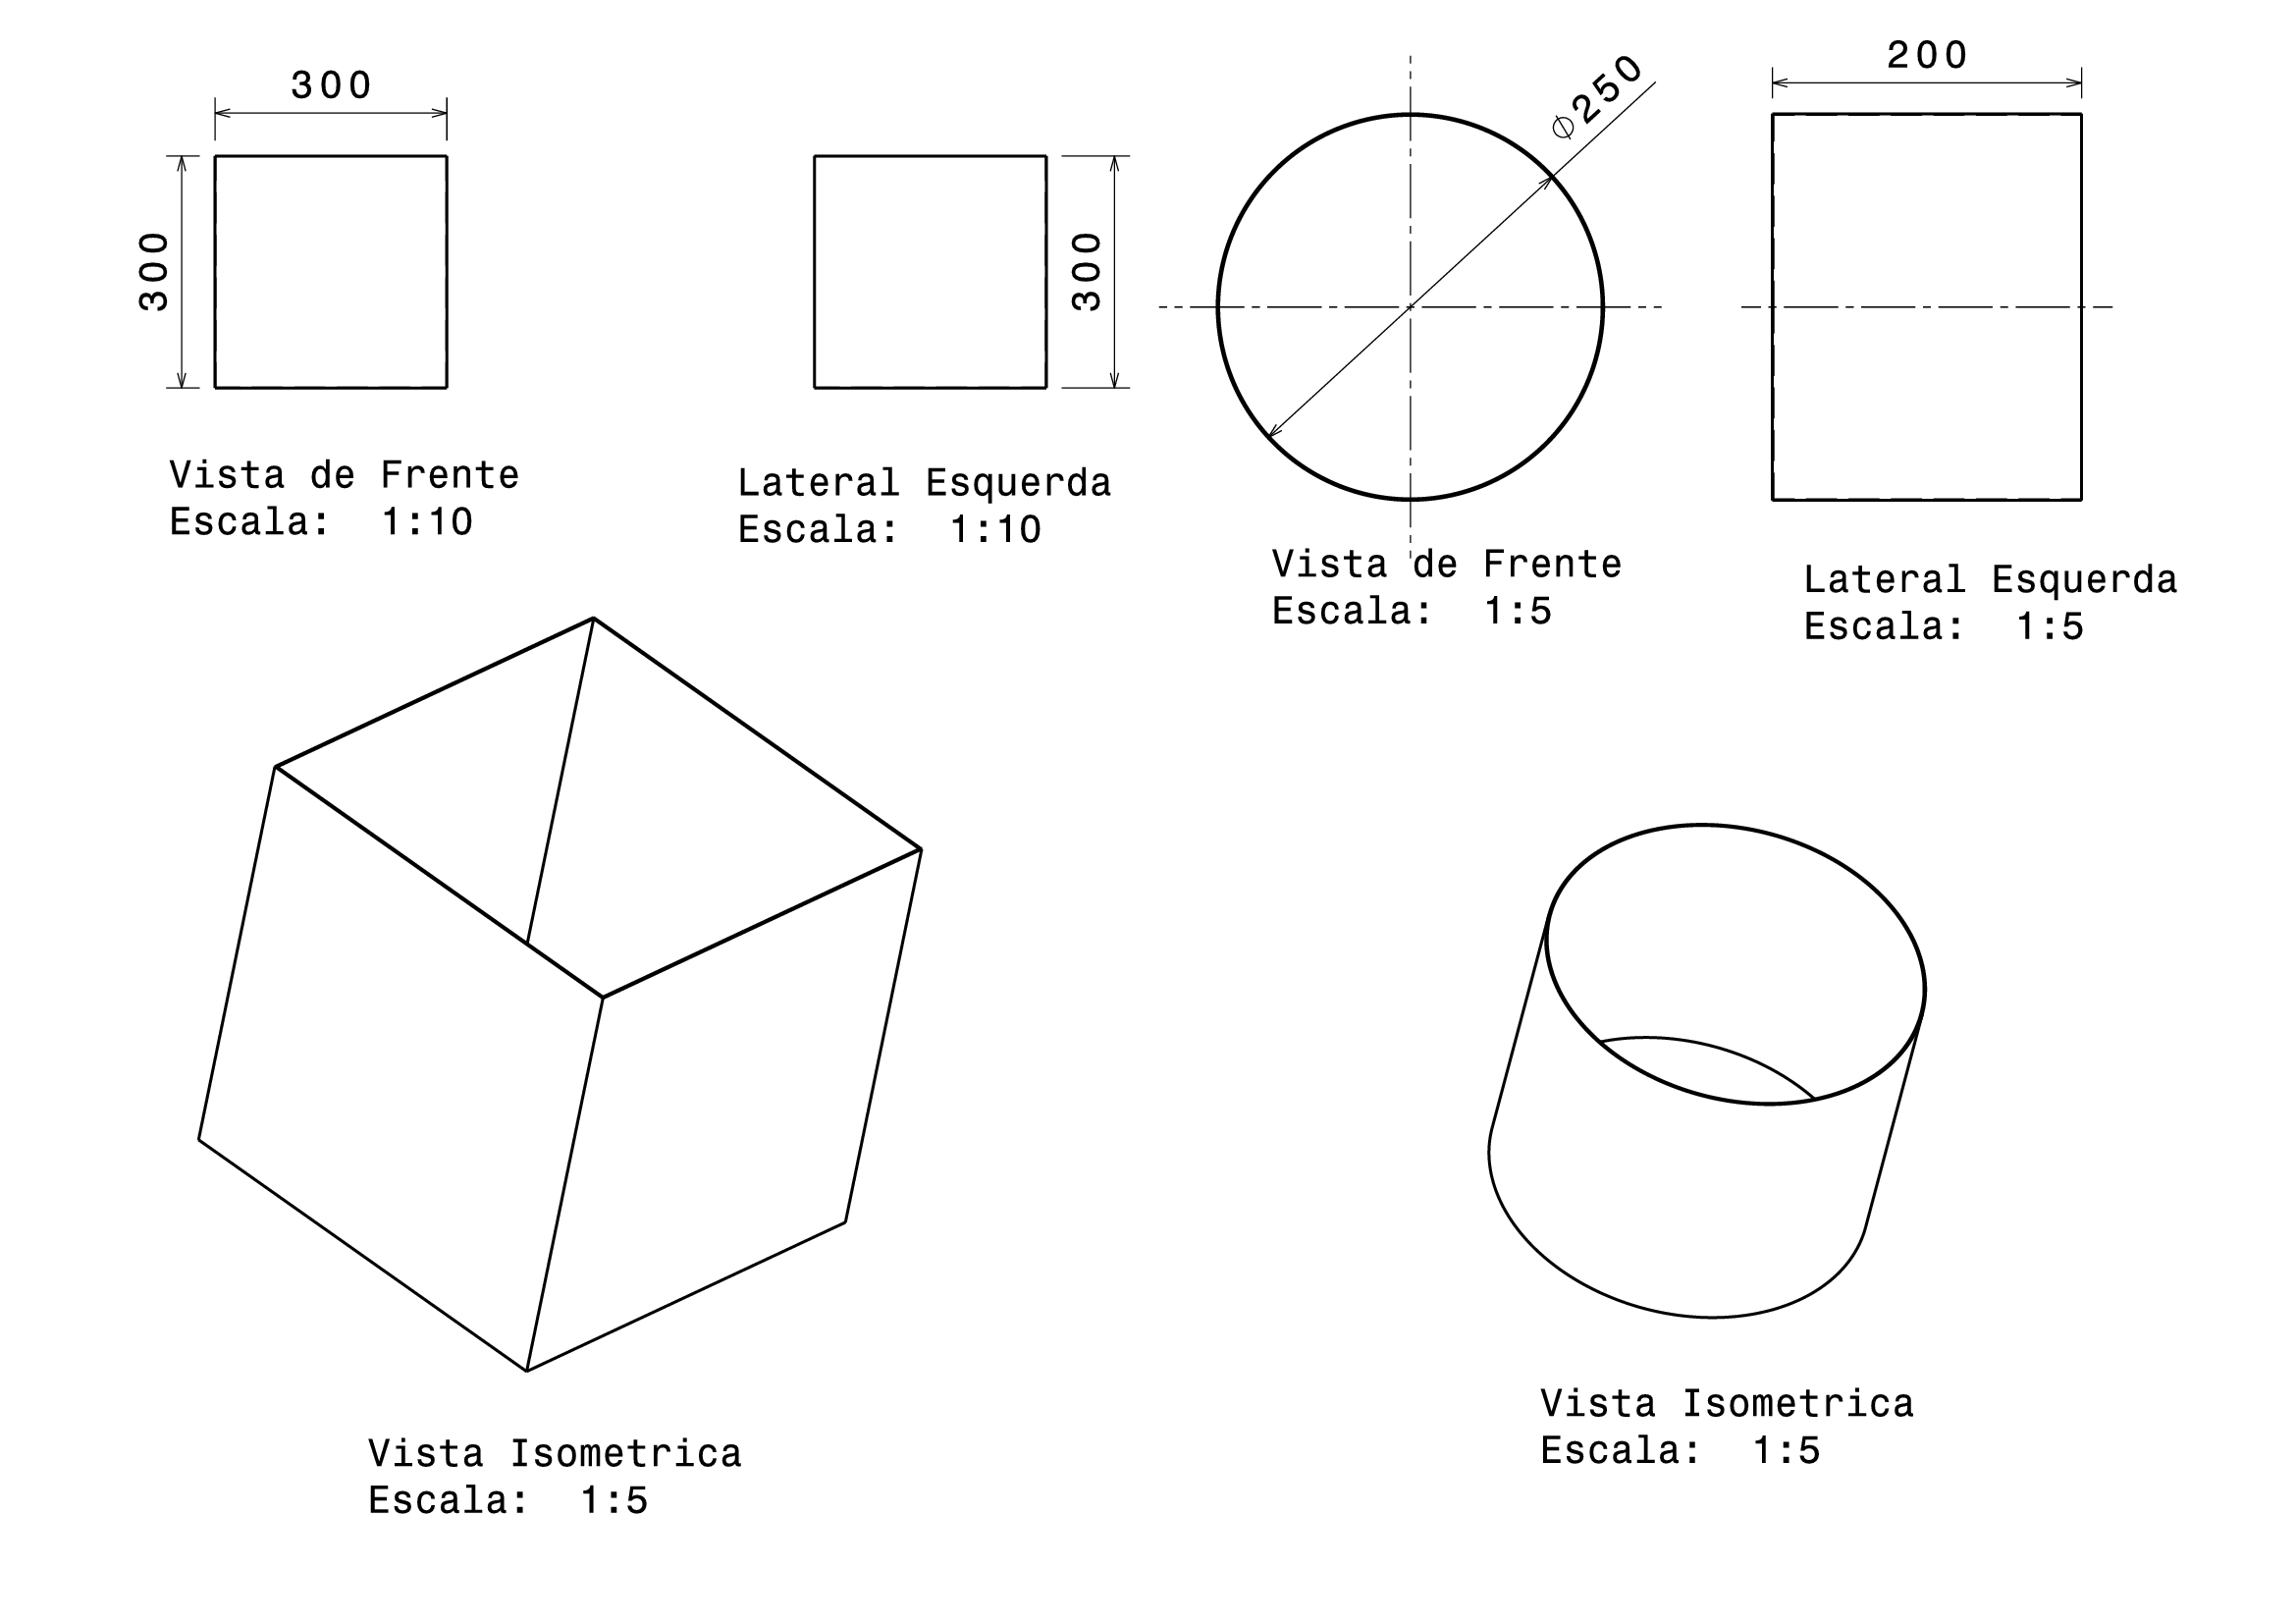
\includegraphics[scale=0.15]{figuras/caixas.png}
\caption{Dimensões dos elementos estruturais internos}
\end{figure}

\subsection{Materiais principais}

O material estrutural tem como objetivo resistir aos esforços durante a utilização da transportadora de órgãos. As cargas de ocorrências durante sua utilização são puramente estáticas, além disso, o projeto deve conciliar baixo custo com baixo peso. Portanto, uma boa opção é o metalon, um aço carbono com costura de baixo custo comumente utilizado em estruturas mecânicas.

\begin{figure}[H]
\centering
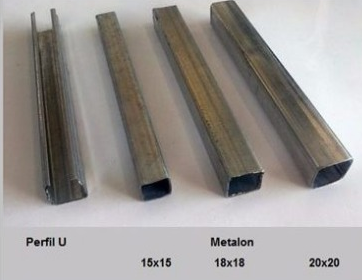
\includegraphics[scale=1]{figuras/metalon.png}
\caption{Perfis de Metalon}
\end{figure}

Para a caixa de alocação de órgãos, foi escolhido o aço inox, devido suas propriedades anticorrosivas e térmicas, aliadas ao baixo custo e maior facilidade de aquisição quando comparado com o aço cirúrgico.

\begin{figure}[H]
\centering
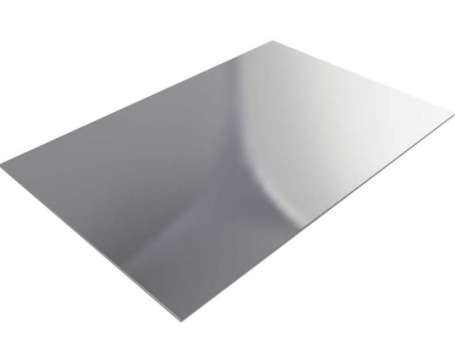
\includegraphics[scale=0.8]{figuras/chapainox.png}
\caption{Chapa de Aço Inox 304}
\end{figure}

A carenagem em volta da estrutura será feita de Policloreto de Vinila (PVC), por ser um material leve e de fácil maneabilidade.

\begin{figure}[H]
\centering
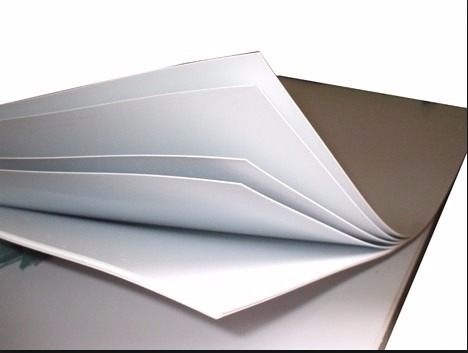
\includegraphics[scale=0.8]{figuras/pvc.png}
\caption{Chapas de Policloreto de Vinila}
\end{figure}

\subsection{Requisitos}

\subsubsection{Requisitos Funcionais}
\begin{itemize}
\item Ser capaz de armazenar o órgão hermeticamente
\item Comportar todos os outros subsistemas
\item Ser móvel e carregável
\item Todas as partes internas do compartimento de carga devem ser capazes de passar por processo de esterilização
\end{itemize}

\subsubsection{Requisitos não-funcionais}

\begin{itemize}
\item Possuir compartimento que possa ser completamente vedado
\item Possuir sistema de rodas para movimentação em solo e alças para carregamento manual
\item Pesar um máximo de 40 kg
\item As peças que serão refrigeradas devem ser resistentes a corrosão
\item Os elementos responsáveis por suportar cargas devem ter resistência para isto
\item O sistema de rodas deve ser capaz de fácil anexagem e desanexagem
\item O compartimento de carga de órgãos deve ser facilmente anexado e desanexado em seu local
\end{itemize}

\subsection{Desafios Técnicos}

\subsubsection{Isolamento térmico da câmara}
Para ajudar a manter uma baixa temperatura estável na câmara fria, é necessário que haja um isolamento térmico em volta do compartimento resfriado. Para isto será feito um revestimento de poliestireno expandido (isopor) ou espuma de poliuretano ao redor da câmara fria.

\subsubsection{Esterilização do sistema}
De acordo com as normas o compartimento no qual o órgão estará contido deve ser esterilizado, portanto deve ser capaz de fácil montagem e desmontagem, o cria um desafio para a fabricação de um compartimento que seja facilmente retirado quando necessário, mas ao mesmo tempo deve estar fixo durante todo o transporte do órgão. Em vista disso, o compartimento estará anexado a estrutura através de peças centralizadoras de seção quadrada com as dimensões da câmara fria e um furo cujo diâmetro é o mesmo do compartimento de carga.
         
\subsubsection{Mobilidade do sistema}
A transportadora possui fácil mobilidade como requisito, o que traz como desafio técnico como será feito o sistema de mobilização de modo estável. A solução que será adotada consiste em módulo que pode ser anexado e desanexado da estrutura principal. Deste modo, quando necessário colocar a transportadora em cima de uma bancada ou algo semelhante, é possível desanexar o módulo de mobilização. O módulo possuirá rodas de baixa vibração e boa capacidade de carga com travas.